%%%%%%%%%%%%%%%%%%%%%%%%%%%%%%%%%%%%%%%%%%%%%%%%%%%%%%%
% MatPlotLib and Random Cheat Sheet
%
% Edited by Michelle Cristina de Sousa Baltazar
%
% http://matplotlib.org/api/pyplot_summary.html
% http://matplotlib.org/users/pyplot_tutorial.html
%
%%%%%%%%%%%%%%%%%%%%%%%%%%%%%%%%%%%%%%%%%%%%%%%%%%%%%%%

\documentclass{article}
\usepackage[landscape]{geometry}
\usepackage{url}
\usepackage{multicol}
\usepackage{multirow}
\usepackage{amsmath}
\usepackage{amsfonts}
\usepackage{booktabs}
\usepackage{tikz}
\usetikzlibrary{decorations.pathmorphing}
\usepackage{amsmath,amssymb}

\usepackage{colortbl}
\usepackage{xcolor}
\usepackage{mathtools}
\usepackage{amsmath,amssymb}
\usepackage{enumitem}

\title{Soils and Aggregates Symbol Cheat Sheet}
%\usepackage[brazilian]{babel}
\usepackage[utf8]{inputenc}

\advance\topmargin-.9in
\advance\textheight3in
\advance\textwidth3in
\advance\oddsidemargin-1.2in
\advance\evensidemargin-1.2in
\parindent0pt
\parskip2pt
\newcommand{\hr}{\centerline{\rule{3.5in}{1pt}}}
%\colorbox[HTML]{e4e4e4}{\makebox[\textwidth-2\fboxsep][l]{texto}
\begin{document}

\begin{center}{\huge{\textbf{Soils, Aggregates, and Asphalt Cheat Sheet}}}\\
{\large By: Dr. Armen Amirkhanian, P.E.}
\end{center}
\begin{multicols*}{3}

\tikzstyle{mybox} = [draw=black, fill=white, very thick,
    rectangle, rounded corners, inner sep=10pt, inner ysep=10pt]
\tikzstyle{fancytitle} =[fill=black, text=white, font=\bfseries]

\begin{tikzpicture}
\node [mybox] (box){%
    \begin{minipage}{0.3\textwidth}
		
\begin{tabular}{lcl}
$e$          & (decimal) & Voids ratio                \\
$n$          & \%        & Porosity                   \\
$w$          & \%        & Water content              \\
$S$          & \%        & Degree of saturation       \\
$V_a$        & L$^3$     & Volume of air              \\
$V_s$        & L$^3$     & Volume of solids           \\
$V_t$        & L$^3$     & Volume, total              \\
$V_v$        & L$^3$     & Volume of voids            \\
$V_w$        & L$^3$     & Volume of water            \\
$M_s$        & M         & Mass of solids             \\
$M_w$        & M         & Mass of water              \\
$\rho$       & M/L$^3$   & Wet or moist total density \\
$\rho '$     & M/L$^3$   & Buoyant density            \\
$\rho_d$     & M/L$^3$   & Dry density                \\
$\rho_s$     & M/L$^3$   & Solids density             \\
$\rho_{sat}$ & M/L$^3$   & Saturated density          \\
$\rho_w$     & M/L$^3$   & Water density             
\end{tabular}

    \end{minipage}
};
%------------ CAIXA RANDOM ---------------------
\node[fancytitle, right=10pt] at (box.north west) {Soil Phase Variables};
\end{tikzpicture}


%------------ CONTEÚDO CAIXA MatPlotLib ---------------
\begin{tikzpicture}
\node [mybox] (box){%
    \begin{minipage}{0.3\textwidth}

\begin{align*}
e&=\dfrac{V_v}{V_s} &            \rho_s&=\dfrac{M_s}{V_s}        \\
n&=\dfrac{V_v}{V_t}\times 100 & \rho_w&=\dfrac{M_w}{V_w}         \\
S&=\dfrac{V_w}{V_v}\times 100 & \rho_d&=\dfrac{M_s}{V_t}         \\
w&=\dfrac{M_w}{M_s}\times 100 & \rho_{sat}&=\dfrac{M_s+M_w}{V_t} \\
\rho&=\dfrac{M_t}{V_t}        & \rho ' &=\rho_{sat}-\rho_w      
\end{align*}

    \end{minipage}
};
%------------ CAIXA PRELIMINARES ---------------------
\node[fancytitle, right=10pt] at (box.north west) {Soil Phase Equations};
\end{tikzpicture}
%------------ CONTEUDO EXEMPLO BASICO ---------------------
\begin{tikzpicture}
\node [mybox] (box){%
    \begin{minipage}{0.3\textwidth}
    	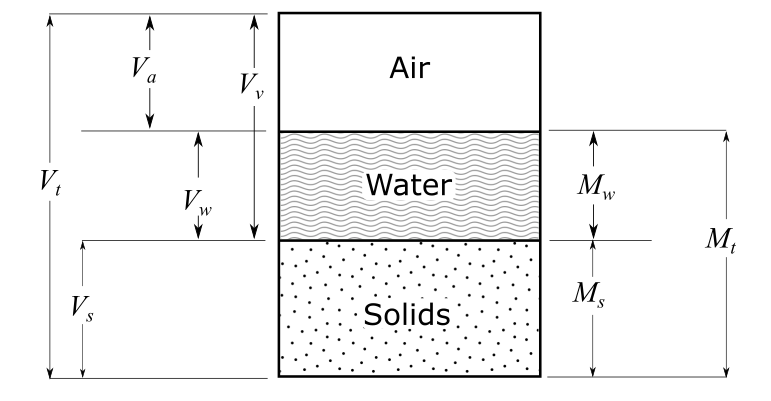
\includegraphics[width=0.99\textwidth]{Three_Phase_soil_diagram.png}
    \end{minipage}
};
%------------ EXEMPLO BASICO BOX ---------------------
\node[fancytitle, right=10pt] at (box.north west) {Soil Phase Schematic};
\end{tikzpicture}
%------------ CONTEUDO DOIS EIXOS ---------------------
\begin{tikzpicture}
\node [mybox] (box){%
    \begin{minipage}{0.3\textwidth}
		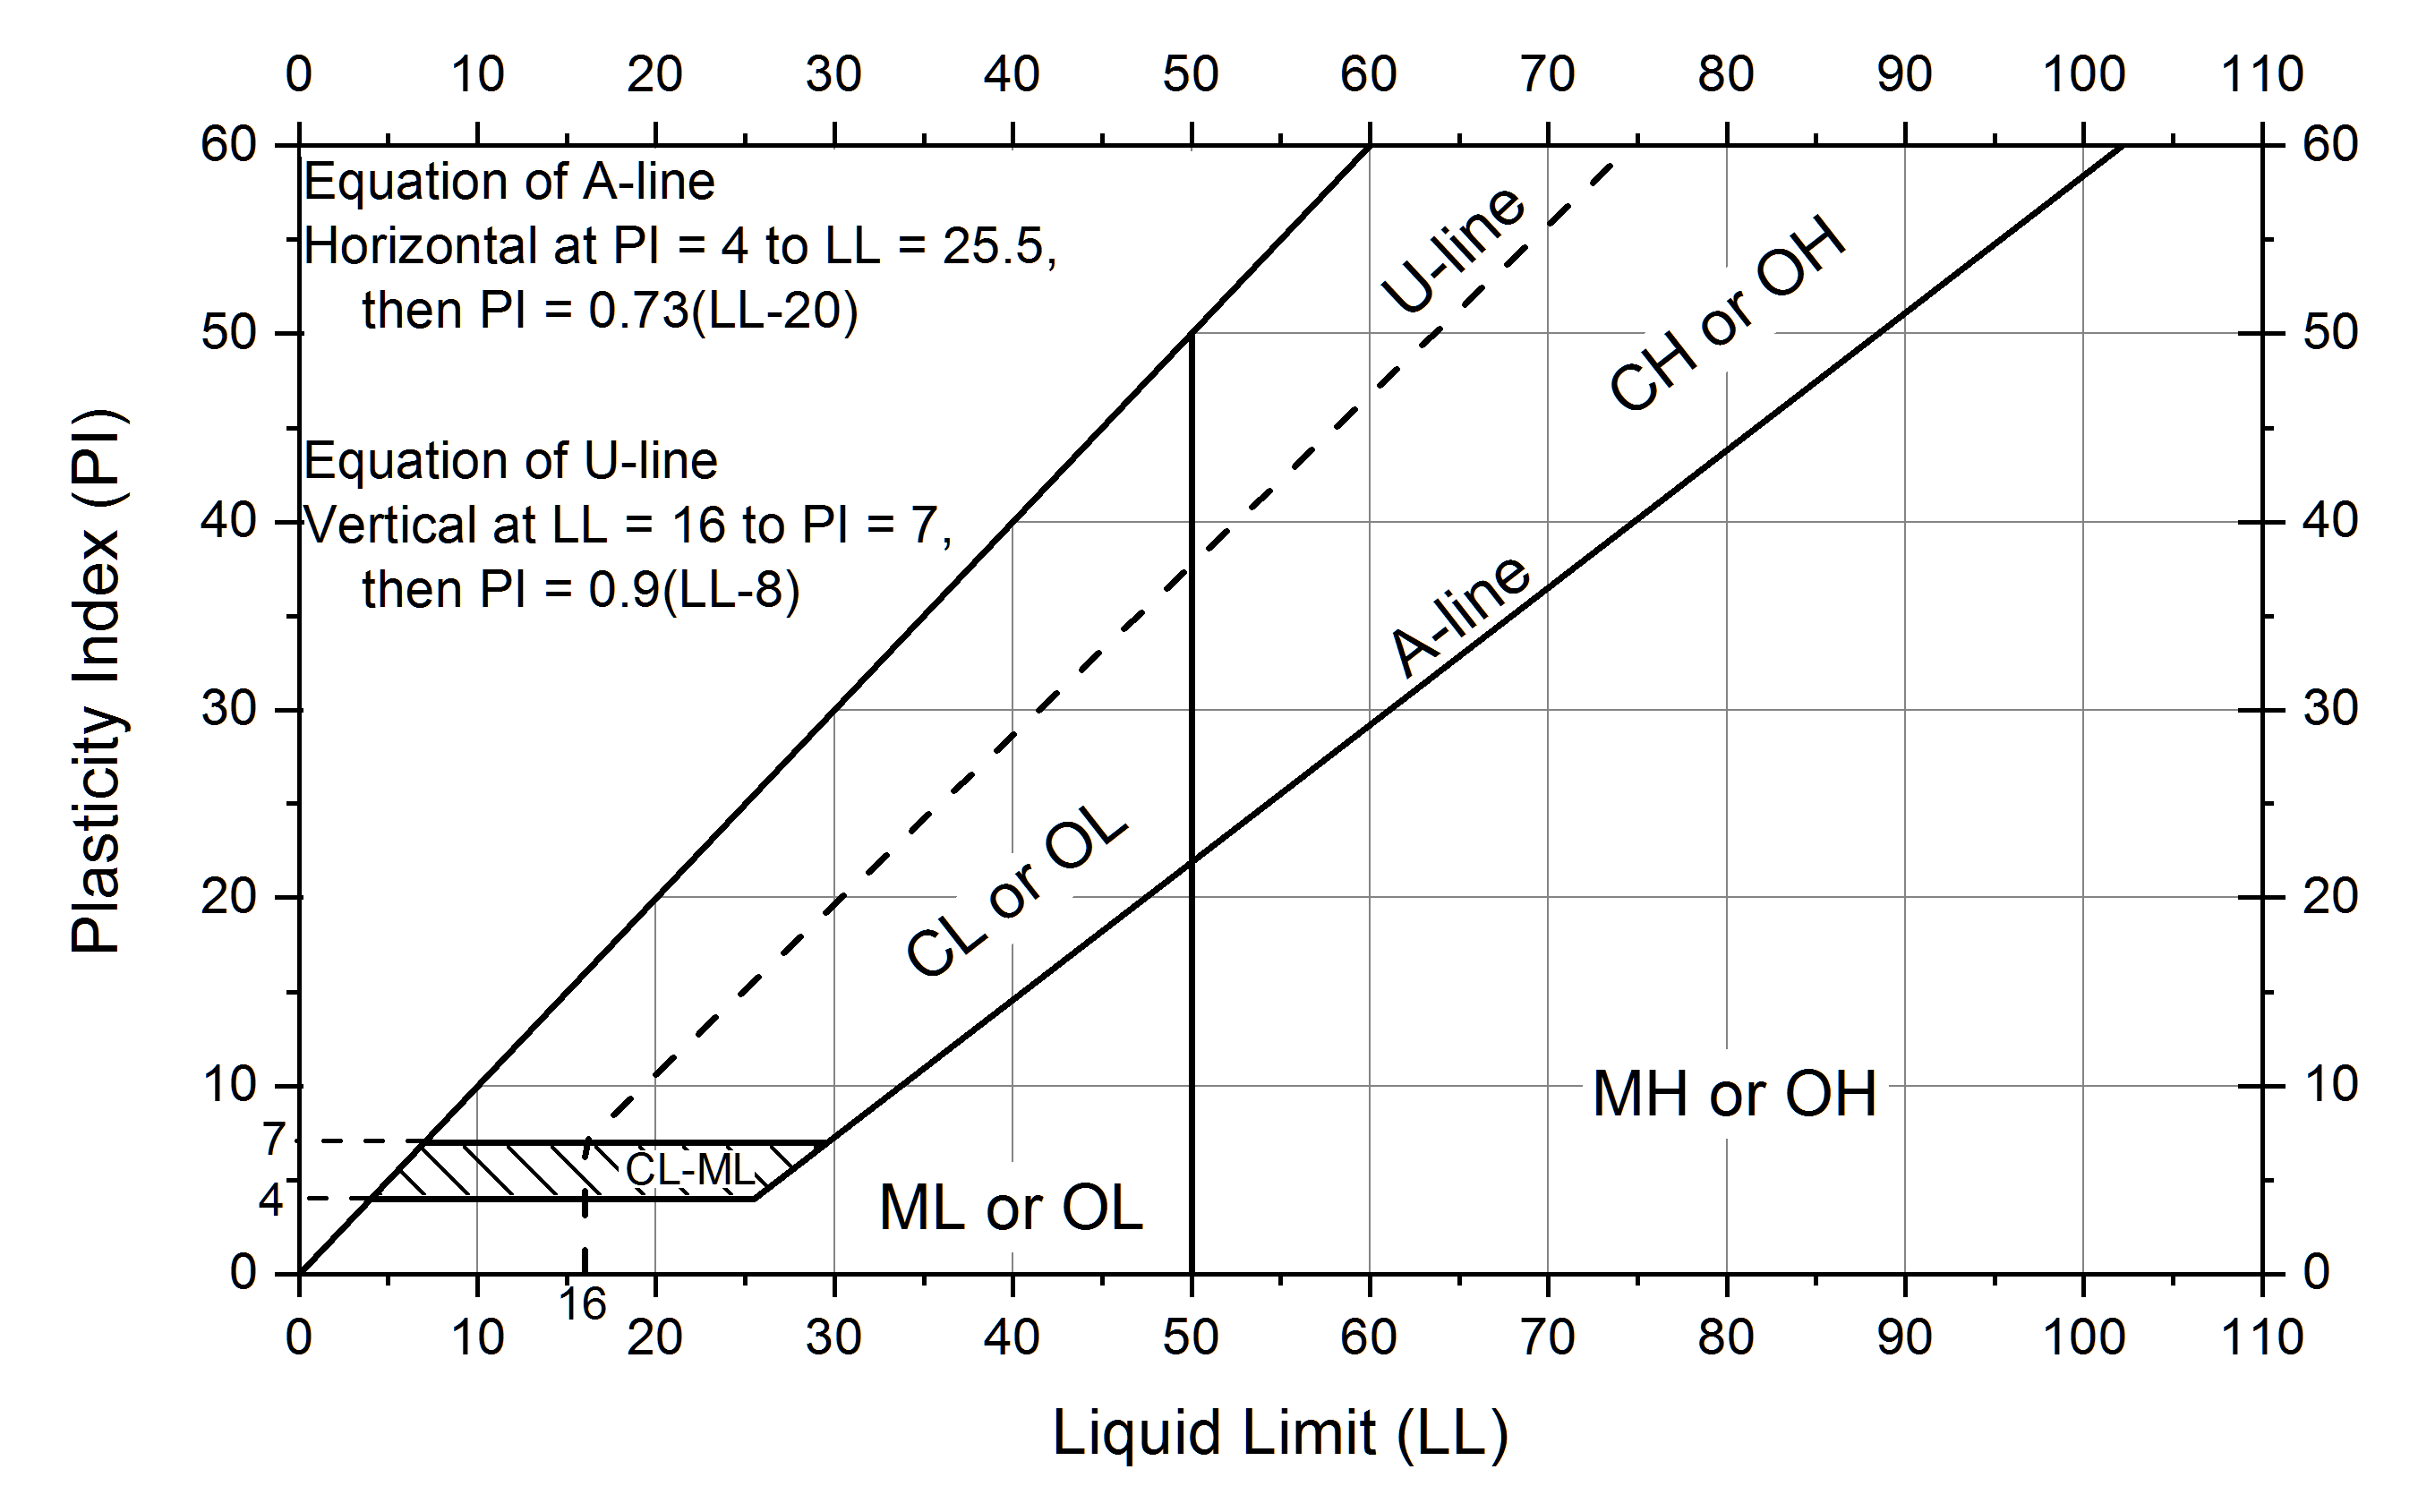
\includegraphics[width=0.99\textwidth]{Casagrande_Chart.png}
    \end{minipage}
};
%------------ DOIS EIXOS BOX ---------------------
\node[fancytitle, right=10pt] at (box.north west) {Casagrande Plasticity Chart};
\end{tikzpicture}
%------------ CONTEÚDO COMANDOS DE TEXTO ---------------------
\begin{tikzpicture}
\node [mybox] (box){%
    \begin{minipage}{0.3\textwidth}
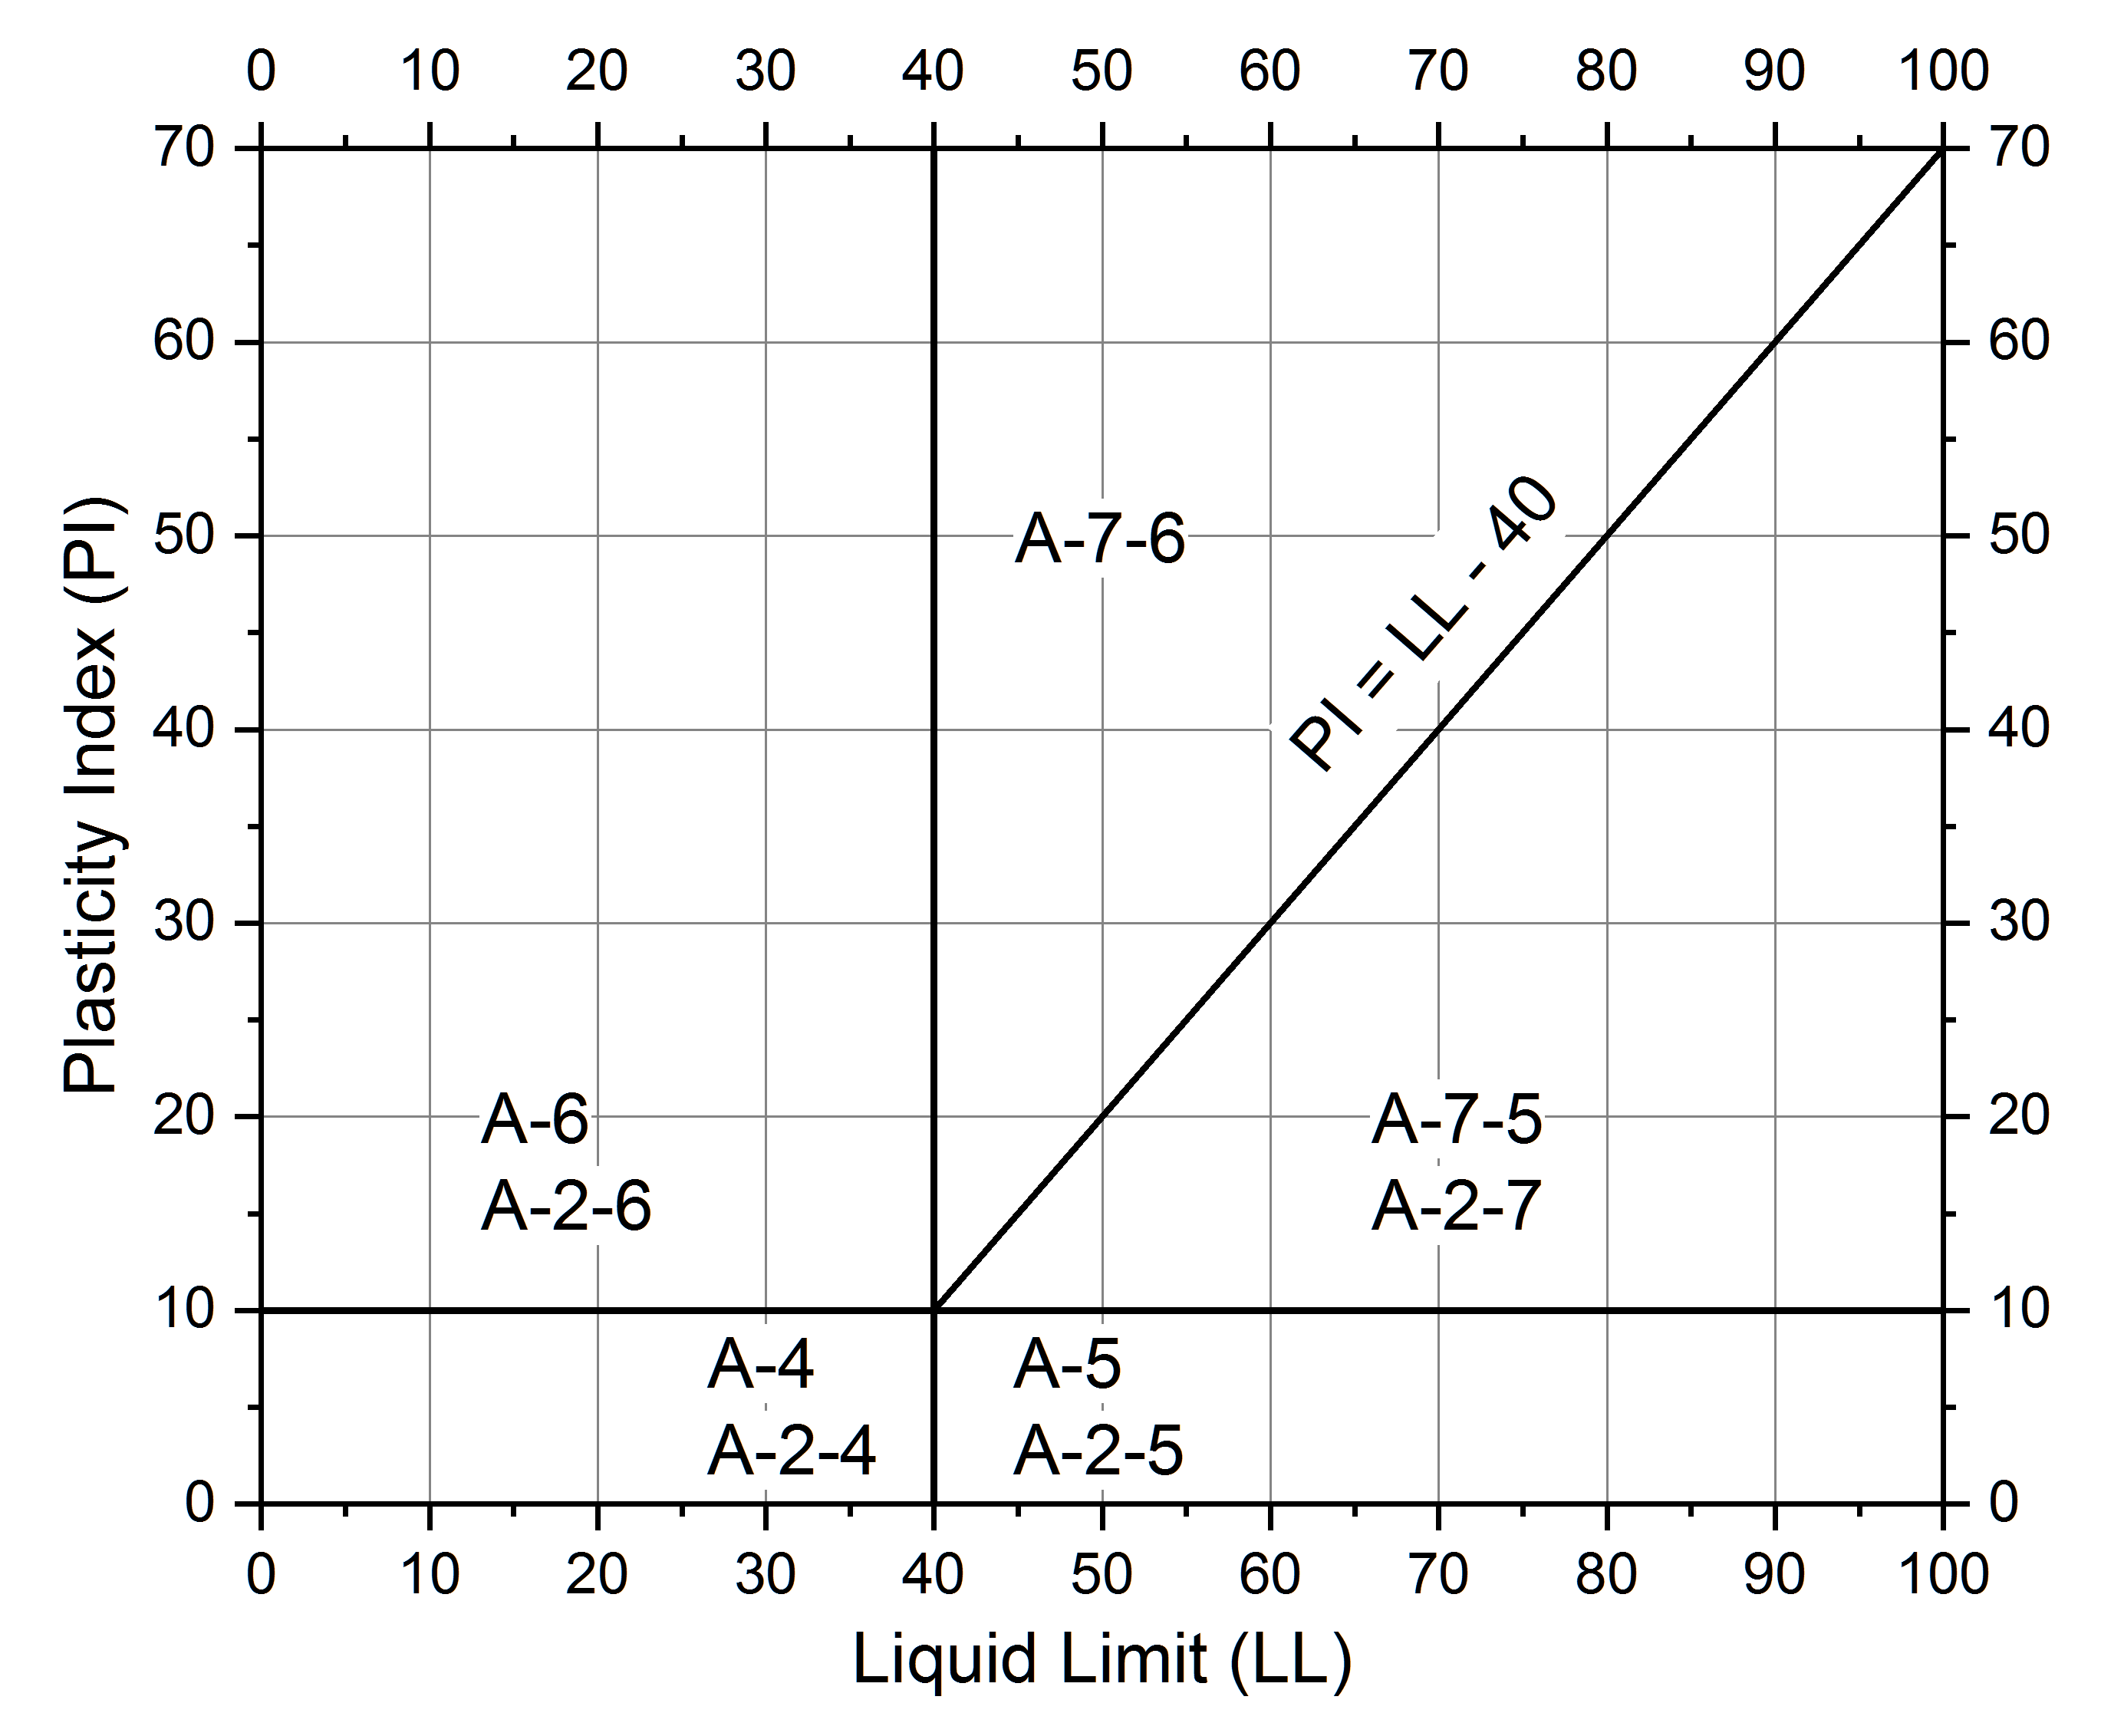
\includegraphics[width=0.99\textwidth]{AASHTO.png}


    \end{minipage}
};
%------------ COMANDOS DE TEXTO BOX ---------------------
\node[fancytitle, right=10pt] at (box.north west) {AASHTO M145 Silt-Clay Materials};
\end{tikzpicture}
%------------ CONTEUDO PROPRIEDADES ---------------------


\begin{tikzpicture}
\node [mybox] (box){%
    \begin{minipage}{0.59\textwidth}
\centering
\begin{tabular}{cccclcccccc}
\hline
\multirow{3}{*}{\begin{tabular}[c]{@{}c@{}}Design\\ ESALs,\\ million\end{tabular}} & \multicolumn{3}{c}{\multirow{2}{*}{\begin{tabular}[c]{@{}c@{}}Required\\ Compaction, \%\end{tabular}}} &  & \multicolumn{4}{c}{VMA, min \%} &  &  \\ \cline{6-9}
 & \multicolumn{3}{c}{} &  & \multicolumn{4}{c}{NMAS, mm} & VFA Range, & Dust/Binder \\ \cline{2-4} \cline{6-9}
 & $N_i$ & $N_d$ & $N_m$ &  & 19.0 & 12.5 & 9.5 & 4.75 & \% & Ratio Range \\ \hline
$<$0.3 & $\leq$91.5 & 96 & $\leq$98 &  & 13 & 14 & 15 & 16 & 70--80 & 0.6--1.2 \\
0.3 to $<$3 & $\leq$90.5 & 96 & $\leq$98 &  & 13 & 14 & 15 & 16 & 65--78 & 0.6--1.2 \\
3 to $<$10 & $\leq$89.0 & 96 & $\leq$98 &  & 13 & 14 & 15 & 16 & 65--75 & 0.6--1.2 \\
10 to $<$30 & $\leq$89.0 & 96 & $\leq$98 &  & 13 & 14 & 15 & 16 & 65--75 & 0.6--1.2 \\
$\geq$30 & $\leq$89.0 & 96 & $\leq$98 &  & 13 & 14 & 15 & 16 & 65--75 & 0.6--1.2 \\ \hline
\multicolumn{11}{l}{\textit{This table does not include any of the footnotes found in AASHTO M323 }}\\
\multicolumn{11}{l}{\textit{and should only be used as a general reference.}}
\end{tabular}

\end{minipage}
};

\node[fancytitle, right=10pt] at (box.north west) {Superpave HMA Design Req. (adapted from AASHTO M323)};
\end{tikzpicture}

%------------ CONTEÚDO COMANDOS DE TEXTO ---------------------
\begin{tikzpicture}
\node [mybox] (box){%
    \begin{minipage}{0.25\textwidth}
\begin{align*}
    VMA &= \left(1-\dfrac{G_{mb}\left(1-P_b\right)}{G_{sb}}\right)\times 100 \\
    VTM &= \left(1-\dfrac{G_{mb}}{G_{mm}}\right)\times 100\\
    VFA &= \dfrac{VMA-VTM}{VMA}\times 100 
\end{align*}


    \end{minipage}
};
%------------ COMANDOS DE TEXTO BOX ---------------------
\node[fancytitle, right=10pt] at (box.north west) {Asphalt Concrete Vol. Equations};
\end{tikzpicture}
%------------ CONTEUDO PROPRIEDADES ---------------------


%------------ CONTEÚDO COMANDOS DE TEXTO ---------------------
\begin{tikzpicture}
\node [mybox] (box){%
    \begin{minipage}{0.25\textwidth}
\begin{align*}
    G_{se} &= \dfrac{1-P_b}{\dfrac{1}{G_{mm}}-\dfrac{P_b}{G_b}}\\
    G_{se} &= G_{sb}+0.8\left(G_{sa}-G_{sb}\right)\quad\mathrm{estimate}\\
    P_{ba} &= \dfrac{G_{se}-G_{sb}}{G_{sb}G_{se}}G_b\times 100\\
    P_{be} &= P_b - \dfrac{P_{ba}}{100}P_{agg}\\
    C^* &= \dfrac{G_{mb}}{G_{mm}}\times 100
\end{align*}
*percent compaction of an asphalt concrete


    \end{minipage}
};
%------------ COMANDOS DE TEXTO BOX ---------------------
\node[fancytitle, right=10pt] at (box.north west) {Asphalt Concrete Misc. Equations};
\end{tikzpicture}
%------------ CONTEUDO PROPRIEDADES ---------------------

%------------ CONTEÚDO COMANDOS DE TEXTO ---------------------
\begin{tikzpicture}
\node [mybox] (box){%
    \begin{minipage}{0.25\textwidth}
We ignore the acceleration of gravity for all unit weight/specific gravity calculations.\\~\\
Good luck, you got this!


    \end{minipage}
};
%------------ COMANDOS DE TEXTO BOX ---------------------
\node[fancytitle, right=10pt] at (box.north west) {Misc. Items};
\end{tikzpicture}
%------------ CONTEUDO PROPRIEDADES ---------------------

\end{multicols*}
\end{document}
Contact GitHub API Training Shop Blog About
© 2016 GitHub, Inc. Terms Privacy Security Status Help